\documentclass[10pt,letterpaper]{article}
\usepackage[utf8]{inputenc}
\usepackage[T1,T2A]{fontenc}
\title{EV 2.3 Explicar los arreglos y parametros de los amplificadores clase B}
\author{Ascencio De Leon Agustin}
\usepackage[spanish]{babel}
\usepackage{graphicx}
\graphicspath{{IMAGENES3/}}
\usepackage[left=2.5cm,top=2.5cm,bottom=3cm,right=2.5cm]{geometry}


\begin{document}
\maketitle
\begin{figure}[h!]
\centering 
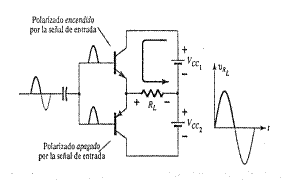
\includegraphics[scale=.8]{55}
\end{figure}
\newpage 
\section{Funcionamiento en clase B}
En algunas aplicaciones, como son los sistemas alimentados son necesarios un bajo consumo de corriente y un alto rendimiento de la etapa. Este hecho condujo a otras formas de funcionamiento. El funcionamiento en clase B de un transistor conlleva que la corriente del colector circule solamente 180° del ciclo de señal, lo que implica que el punto Q ubique aproximadamente en el punto de corte en ambas rectas de carga, la de corriente continua y la de señal. Las ventajas que ofrece el funcionamiento en clase B son un menor consumo de corriente y un mayor rendimiento.
\linebreak
\begin{figure}
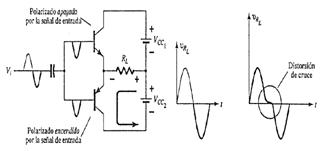
\includegraphics[scale=.9]{56}
\end{figure}
\linebreak
\subsection{ Circuito en contrafase}
Cuando un transistor funciona en clase B sólo amplifica la mitad de un ciclo. Para evitar la distorsión, se emplean dos transistores dispuestos en contrafase (conocido en inglés como push-pu11). Este hecho significa que uno de los transistores conduce durante un semiciclo y el otro transistor durante el otro. Con los circuitos en contrafase se pueden construir amplificadores clase B que tengan baja distorsión y gran poten­cia en la carga.
\section{Recta de carga para continua}
Al no haber resistencia para continua en los circuitos de colector o de emisor de la figura anterior, la corriente de saturación para continua es infinita. Este hecho significa que la recta de carga para continua es vertical. Si esta situación le peligrosa, no se equivoca. La mayor dificultad al diseñar un amplificador de clase B es el situar de forma estable el punto Q en el punto de corte. Cualquier descenso significativo de VBE con la temperatura puede elevar el punto Q sobre la recta de carga para continuo hacia corrientes grandes, con el consiguiente peligro.
\section{Recta de carga para señal}
La figura muestra la recta de carga para señal. Cuando alguno de los transistores está conduciendo, el punto de trabajo del transistor que conduce se eleva sobre la recta de carga para señal. El punto de trabajo del otro transistor se mantiene en corte. La variación de tensión el transistor que está conduciendo puede recorrer todo el camino desde corte a saturación. En el siguiente semiciclo, el otro transistor actuará de la misma forma. Este hecho significa que la máxima salida pico a pico no recortada es igual a

MPP=VCC

\section{Análisis para señal}
La figura muestra el circuito equivalente para señal del transistor del en conducción. Dicho circuito es casi idéntico al de un seguidor emisor en clase A. La ganancia de tensión con carga es

La impedancia de entrada de la base

\end{document}